\documentclass[tikz,border=3pt]{standalone}
\usepackage[utf8]{inputenc}
\usepackage[T1]{fontenc}
\usepackage{lmodern}
\renewcommand{\familydefault}{\sfdefault}
\usepackage{sansmath}\sansmath
\usepackage{chemfig}
\usepackage{pgfplots}\pgfplotsset{compat=1.18,/pgf/number format/use comma,/pgf/number format/1000 sep={.}}
\usetikzlibrary{arrows.meta,calc,positioning,decorations.pathmorphing,patterns}
% paleta del sitio
\definecolor{nar}{HTML}{E8680C}\definecolor{narc}{HTML}{FFB35C}\definecolor{hielo}{HTML}{FFF3E8}
\definecolor{tinta}{HTML}{1D1D1F}\definecolor{gris}{HTML}{6E6E73}\definecolor{lila}{HTML}{7C5CF0}
\definecolor{azul}{HTML}{2F6FD6}\definecolor{menta}{HTML}{17A673}\definecolor{coral}{HTML}{E8342A}
\begin{document}
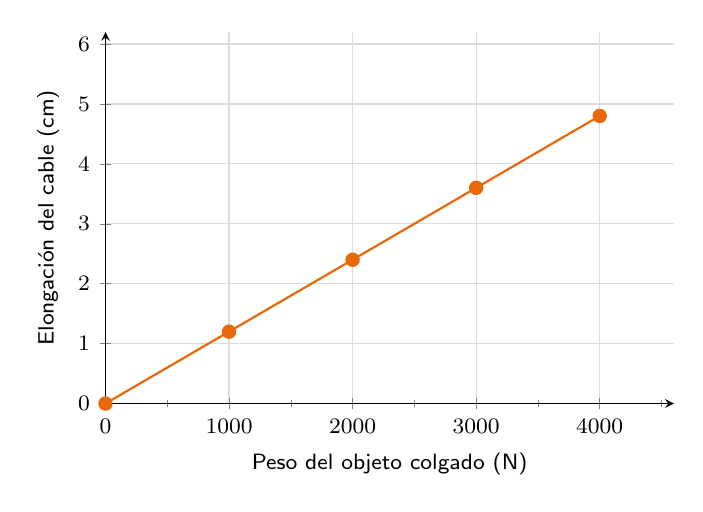
\begin{tikzpicture}[font=\footnotesize]
\begin{axis}[width=8.8cm,height=6.3cm,xmin=0,xmax=4600,ymin=0,ymax=6.2,xtick={0,1000,...,4000},minor xtick={500,1500,...,4500},ytick={0,1,...,6},grid=major,grid style={gris!25},
  scaled x ticks=false,/pgf/number format/1000 sep={},
  xlabel={Peso del objeto colgado (N)},ylabel={Elongación del cable (cm)},axis lines=left,every axis plot/.append style={thick}]
\addplot[nar,mark=*,mark size=2.2pt] coordinates {(0,0)(1000,1.2)(2000,2.4)(3000,3.6)(4000,4.8)};
\end{axis}
\end{tikzpicture}
\end{document}
